%%%%%%%%%%%%%%%%%%%%%%%%%%%%%%%%%%%%%%%%%
% Jacobs Landscape Poster
% LaTeX Template
% Version 1.1 (14/06/14)
%
% Created by:
% Computational Physics and Biophysics Group, Jacobs University
% https://teamwork.jacobs-university.de:8443/confluence/display/CoPandBiG/LaTeX+Poster
% 
% Further modified by:
% Nathaniel Johnston (nathaniel@njohnston.ca)
%
% This template has been downloaded from:
% http://www.LaTeXTemplates.com
%
% License:
% CC BY-NC-SA 3.0 (http://creativecommons.org/licenses/by-nc-sa/3.0/)
%
%%%%%%%%%%%%%%%%%%%%%%%%%%%%%%%%%%%%%%%%%

%----------------------------------------------------------------------------------------
%	PACKAGES AND OTHER DOCUMENT CONFIGURATIONS
%----------------------------------------------------------------------------------------

\documentclass[final]{beamer}

\usepackage[scale=1.24]{beamerposter} % Use the beamerposter package for laying out the poster

\usetheme{confposter} % Use the confposter theme supplied with this template


\definecolor{cpurple}{Gray}{0.15}
\definecolor{corange}{RGB}{246,103,51}

\setbeamercolor{block title}{fg=ngreen,bg=white} % Colors of the block titles
\setbeamercolor{block body}{fg=black,bg=white} % Colors of the body of blocks
\setbeamercolor{block alerted title}{fg=Gray!15,bg=BrickRed!95} % Change the alert block title colors
\setbeamercolor{block alerted body}{fg=black,bg=BrickRed!05} % Change the alert block body colors
% Many more colors are available for use in beamerthemeconfposter.sty

\setbeamercolor{background canvas}{bg=gray!50}

%-----------------------------------------------------------
% Define the column widths and overall poster size
% To set effective sepwid, onecolwid and twocolwid values, first choose how many columns you want and how much separation you want between columns
% In this template, the separation width chosen is 0.024 of the paper width and a 4-column layout
% onecolwid should therefore be (1-(# of columns+1)*sepwid)/# of columns e.g. (1-(4+1)*0.024)/4 = 0.22
% Set twocolwid to be (2*onecolwid)+sepwid = 0.464
% Set threecolwid to be (3*onecolwid)+2*sepwid = 0.708

\newlength{\sepwid}
\newlength{\onecolwid}
\newlength{\twocolwid}
\newlength{\threecolwid}
\setlength{\paperwidth}{48in} % A0 width: 46.8in
\setlength{\paperheight}{36in} % A0 height: 33.1in
\setlength{\sepwid}{0.024\paperwidth} % Separation width (white space) between columns
\setlength{\onecolwid}{0.22\paperwidth} % Width of one column
\setlength{\twocolwid}{0.464\paperwidth} % Width of two columns
\setlength{\threecolwid}{0.708\paperwidth} % Width of three columns
\setlength{\topmargin}{-0.5in} % Reduce the top margin size
%-----------------------------------------------------------

\usepackage{graphicx}  % Required for including images

\usepackage{booktabs} % Top and bottom rules for tables

\usepackage{amsmath}

%----------------------------------------------------------------------------------------
%	TITLE SECTION 
%----------------------------------------------------------------------------------------

\title{\huge Computer model calibration for design, with an application to wind turbine blades} % Poster title

\author{Carl Ehrett\textsuperscript{1,3}, Sez Atamturktur\textsuperscript{2,4}, Andrew Brown\textsuperscript{1,3}, Christopher Kitchens\textsuperscript{1,6}, Mingzhe Jiang\textsuperscript{1,6}, Caleb Arp\textsuperscript{1,6}, Evan Chodora\textsuperscript{1,5}} % Author(s)

\institute{\textsuperscript{1}Clemson University, \textsuperscript{2}Pennsylvania State University, \textsuperscript{3}Dept.\ of Math.\ Sciences, \textsuperscript{4}Dept.\ of Architectural Eng.,\textsuperscript{5}Dept.\ of Civil Eng., 
\textsuperscript{6}Chemical and Biomolecular Eng.} % Institution(s)

%----------------------------------------------------------------------------------------

\begin{document}


\addtobeamertemplate{alertblock end}{}{\vspace*{1ex}} % White space under blocks
\addtobeamertemplate{alertblock alerted end}{}{\vspace*{2ex}} % White space under highlighted (alert) blocks

\setlength{\belowcaptionskip}{1ex} % White space under figures
\setlength\belowdisplayshortskip{2ex} % White space under equations



\begin{frame}[t] % The whole poster is enclosed in one beamer frame

\vspace{-15mm}

\begin{columns}[t] % The whole poster consists of three major columns, the second of which is split into two columns twice - the [t] option aligns each column's content to the top

\begin{column}{\sepwid}\end{column} % Empty spacer column

\begin{column}{\onecolwid} % The first column

%----------------------------------------------------------------------------------------
%	OBJECTIVES
%----------------------------------------------------------------------------------------

%----------------------------------------------------------------------------------------
%	INTRODUCTION
%----------------------------------------------------------------------------------------

\begin{alertblock}{Computer model calibration}
\begin{itemize}
\item Computer models may include unknown inputs that must be estimated\cite{Kennedy2001}. 
These inputs are often estimated by combining simulator output with field data. 

%\item E.g.: a model's output depends upon a physical constant which is unknown. 

\item Calibration is ordinarily thought of as bringing a computer model into agreement with reality.
%\item Previous explorations of computer model calibration have approached calibration as a matter of bringing a computer model into agreement with physical reality.

\end{itemize}

\end{alertblock}

%------------------------------------------------

\begin{alertblock}{Full model}

\begin{itemize}

\item Where $f$ is the true system, $\eta$ the computer model of $f$, $\delta$ the discrepancy $f-\eta$, $\boldsymbol \theta$ the true values of the calibration parameters, $\mathbf x$ the control inputs, and $\boldsymbol \epsilon$ error, we have $f(\mathbf x,\boldsymbol \theta) \equiv f(\mathbf x) = \eta(\mathbf x,\boldsymbol \theta) + \delta(\mathbf x) + \boldsymbol \epsilon$.
%\vspace{-3mm}
%\[
%f(\mathbf x,\boldsymbol \theta) \equiv f(\mathbf x) = \eta(\mathbf x,\boldsymbol \theta) + \delta(\mathbf x) + \boldsymbol \epsilon
%\]
%
%\vspace{-19mm}
\item When $\eta$ is computationally expensive, we use a mean-zero Gaussian process (GP) emulator as a code surrogate.
%
% code surrogate. In the wind turbine application here, we use a mean-zero Gaussian process emulator for this.
%
$\delta$ is also modeled using a mean-zero GP. Both GPs use a power product exponential covariance function: respectively (where $\mathbf x\in\mathbb R^p$, $\boldsymbol\theta\in\mathbb R^q$),
\vspace{-3mm}
%\[
%C_\eta(\!(\mathbf x,\!\boldsymbol\theta),\!(\mathbf x'\!,\!\boldsymbol\theta')\!)\! = \frac1\lambda_\eta \prod_{k=1}^{p}\left(\rho^\eta_k\right)^{\left(x_k -x_k'\right)^2}
%\times
%\prod_{j=1}^{q}\left( \rho^\eta_{p+j}\right)^{\left(\theta_j-\theta_j'\right)^2},
%\]
%\vspace{-5mm}
%\[
%C_\delta(\mathbf x,\mathbf x') = \frac1\lambda_\delta \prod_{k=1}^{p}\left(\rho^\delta_k\right)^{\left(x_k -x_k'\right)^2}
%\]
\begin{align*}
C_\eta(\!(\mathbf x,\!\boldsymbol\theta),\!(\mathbf x'\!,\!\boldsymbol\theta')\!)\! &= \frac1\lambda_\eta \prod_{k=1}^{p}\left(\rho^\eta_k\right)^{\left(x_k -x_k'\right)^2}
\times
\prod_{j=1}^{q}\left( \rho^\eta_{p+j}\right)^{\left(\theta_j-\theta_j'\right)^2},
\\
C_\delta(\mathbf x,\mathbf x') &= \frac1\lambda_\delta \prod_{k=1}^{p}\left(\rho^\delta_k\right)^{\left(x_k -x_k'\right)^2}
\end{align*}

%\vspace{-8mm}
We use the MLEs of $\lambda_\eta$ and $\boldsymbol\rho^\eta$, set $\rho_i^\delta\sim\mathrm{Beta}(1,0.3)$ for all $i$, and set an informative Gamma prior on $\lambda_\delta$ based on what is known \textit{a priori} about the system optimum.

\item Let $\boldsymbol\eta$ be a vector of univariate observations of the computer model at points $\{(\mathbf x_i,\boldsymbol\theta_i)\}_{i=1}^m$ and $\mathbf y$ be a set of ``desired observations'' at points $\{(\mathbf x_i,\boldsymbol\theta_i)\}_{i=m+1}^{m+n}$. Where $\mathcal D=[\boldsymbol\eta^T,\mathbf y^T]^T$, we have $\mathcal D|\boldsymbol \theta,\lambda_\delta,\boldsymbol\rho^\delta\sim\mathrm N(\mathbf0,\mathbf C_{\mathcal D})$, and 
\[
\pi(\boldsymbol\theta,\lambda_\delta,\boldsymbol\rho^\delta|\mathcal D) \propto
\pi(\mathcal D|\boldsymbol\theta,\lambda_\delta,\boldsymbol\rho^\delta)\times
\pi(\boldsymbol\theta) \times
\pi(\lambda_\delta) \times
\pi(\boldsymbol\rho^\delta).
\]
where $\mathbf C_{\mathcal D}$ is given by $C_\eta$, plus $C_\delta$ in the submatrix corresponding to $\mathbf y$. We explore this via MCMC.

\end{itemize}

\end{alertblock} 

%---------------------------------------------------


\begin{alertblock}{Choosing target observations}

\begin{itemize}
\item To optimize, we need targets exceeding achievable results. But for identifiability, targets should be near the model range. To satisfy these constraints,\! we need a rough estimate of the Pareto front.

\item We achieve this by a preliminary round of calibration, with a weak prior on $\lambda_\delta$. This exploits problems of identifiability in the Kennedy-O'Hagan calibration framework\cite{Kennedy2001} to explore the Pareto front.

\item Using the results of preliminary calibration, we select a performance target near the model range.

\end{itemize}

\begin{figure}[h!]
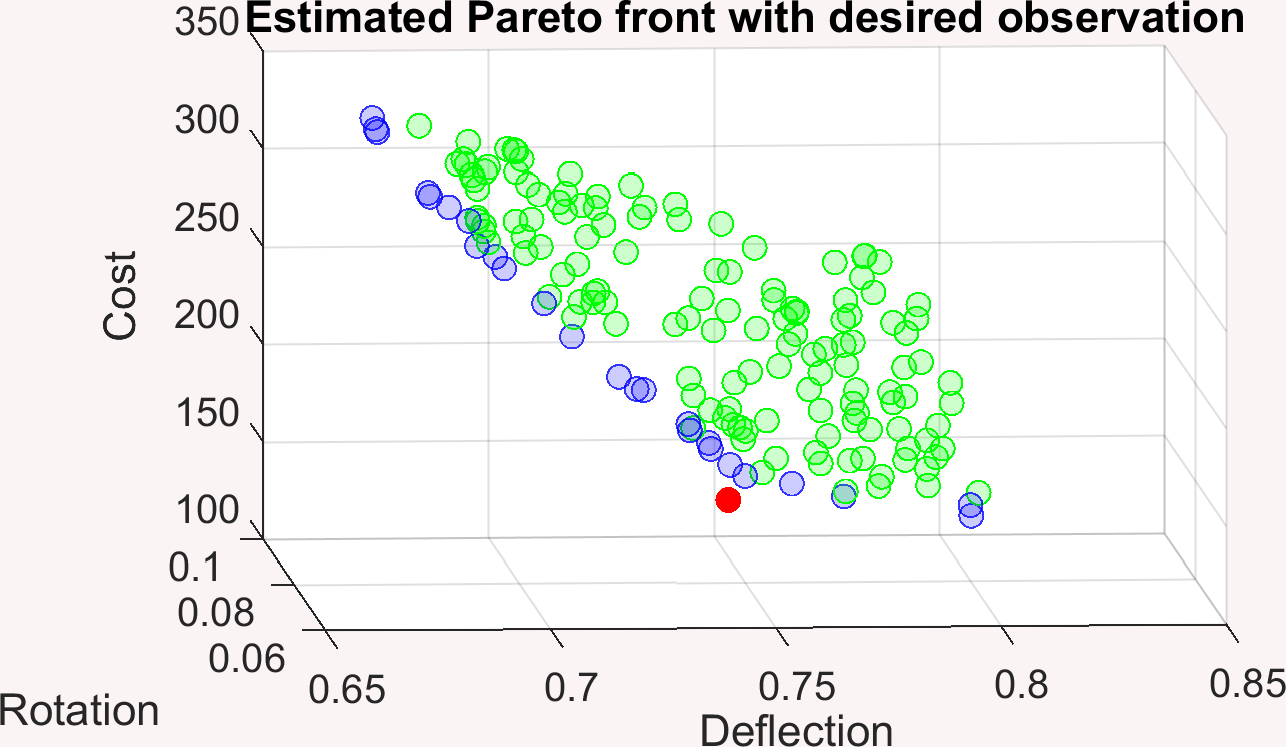
\includegraphics[width=.875\linewidth]{FIG_est_PF_with_des_obs}
%\caption{Wind turbine blade}
\label{est_PF}
\end{figure}


\end{alertblock}




%------------------------------------------------

%\begin{alertblock}{Central idea}
%\begin{itemize}
%\item Previous explorations of computer model calibration have approached calibration as a matter of bringing a computer model into agreement with physical reality.
%
%\item In the present work, we consider computer model calibration as a method for design. 
%
%\item Under this framework, we calibrate a computer model not using physical experimental data, but rather using ``desired data'' which describes the performance one hopes to achieve in the simulated system. 
%
%\end{itemize}
%
%\end{alertblock} 

%----------------------------------------------------------------------------------------

\end{column} % End of the first column



\begin{column}{\sepwid}\end{column} % Empty spacer column

\begin{column}{\twocolwid} % Begin a column which is two columns wide (column 2)

\setbeamercolor{block alerted title}{fg=Gray!15,bg=MidnightBlue!95} % Change the alert block title colors
\setbeamercolor{block alerted body}{fg=black,bg=MidnightBlue!10} % Change the alert block body colors

\begin{alertblock}{Central idea}

Researchers look to computer experiments where physical experimentation is difficult or impossible\cite{Sacks1989,Santner2003a}. Previous explorations of computer model calibration have approached calibration as a matter of bringing a computer model into agreement with physical reality\cite{Bayarri2007,Kennedy2001,Higdon2004,Williams2006}. \textbf{In the present work, we consider computer model calibration as a method for design.} Under this framework, we calibrate a computer model not using physical experimental data, but rather using ``desired observations'' which describe the performance one hopes to achieve in the simulated system. 

\end{alertblock} 

\setbeamercolor{block alerted title}{fg=Gray!15,bg=BrickRed!95} % Change the alert block title colors
\setbeamercolor{block alerted body}{fg=black,bg=BrickRed!05} % Change the alert block body colors

\begin{columns}[t,totalwidth=\twocolwid] % Split up the two columns wide column

\begin{column}{\onecolwid}\vspace{-.6in} % The first column within column 2 (column 2.1)

%----------------------------------------------------------------------------------------
%	MATERIALS
%----------------------------------------------------------------------------------------

\begin{alertblock}{Artificial system example}


\begin{figure}[h!]
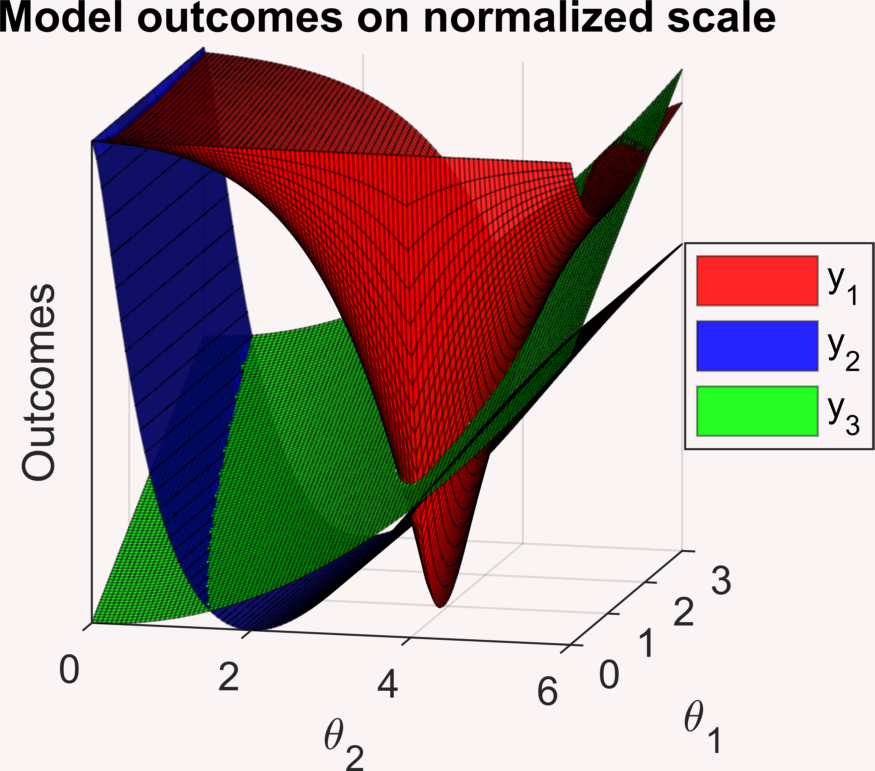
\includegraphics[width=0.6\linewidth]{FIG_toy_sim_model_outputs}
%\caption{Wind turbine blade}
\label{blade}
\end{figure}

\vspace{-10mm}
\begin{itemize}

\item Consider $f:[1.95,2.05]\times[0,3]\times[0,6]\to \mathbb R^3$ where the latter two inputs are treated as calibration parameters. We seek to minimize the three model outputs:
\begin{align*}
f_1(x,\theta_1,\theta_2) &= \left( \theta_1 \exp \left ( - \left( \theta_1 + \lvert \theta_2 - \frac{\pi x}2\rvert \right) \right) + 1 \right)^{-1}\\
f_2(x,\theta_1,\theta_2) &= \left(\theta_2^{x-1} \exp\left(-0.75\theta_2\right)+1\right)^{-1}\\
f_3(x,\theta_1,\theta_2)&=15+2\theta_1+\frac{\theta_2^2}4
\end{align*}

\item Initially, the performance target of $[0,0,0]$ was chosen. To improve the identifiability of the optimal region, we used a preliminary round of calibration to update this to a target of $[0.71,0.71,17.92]$, constant w.r.t.\ $x$.

\end{itemize}
\end{alertblock}


\begin{alertblock}{Artificial example results}


\begin{figure}[h!]
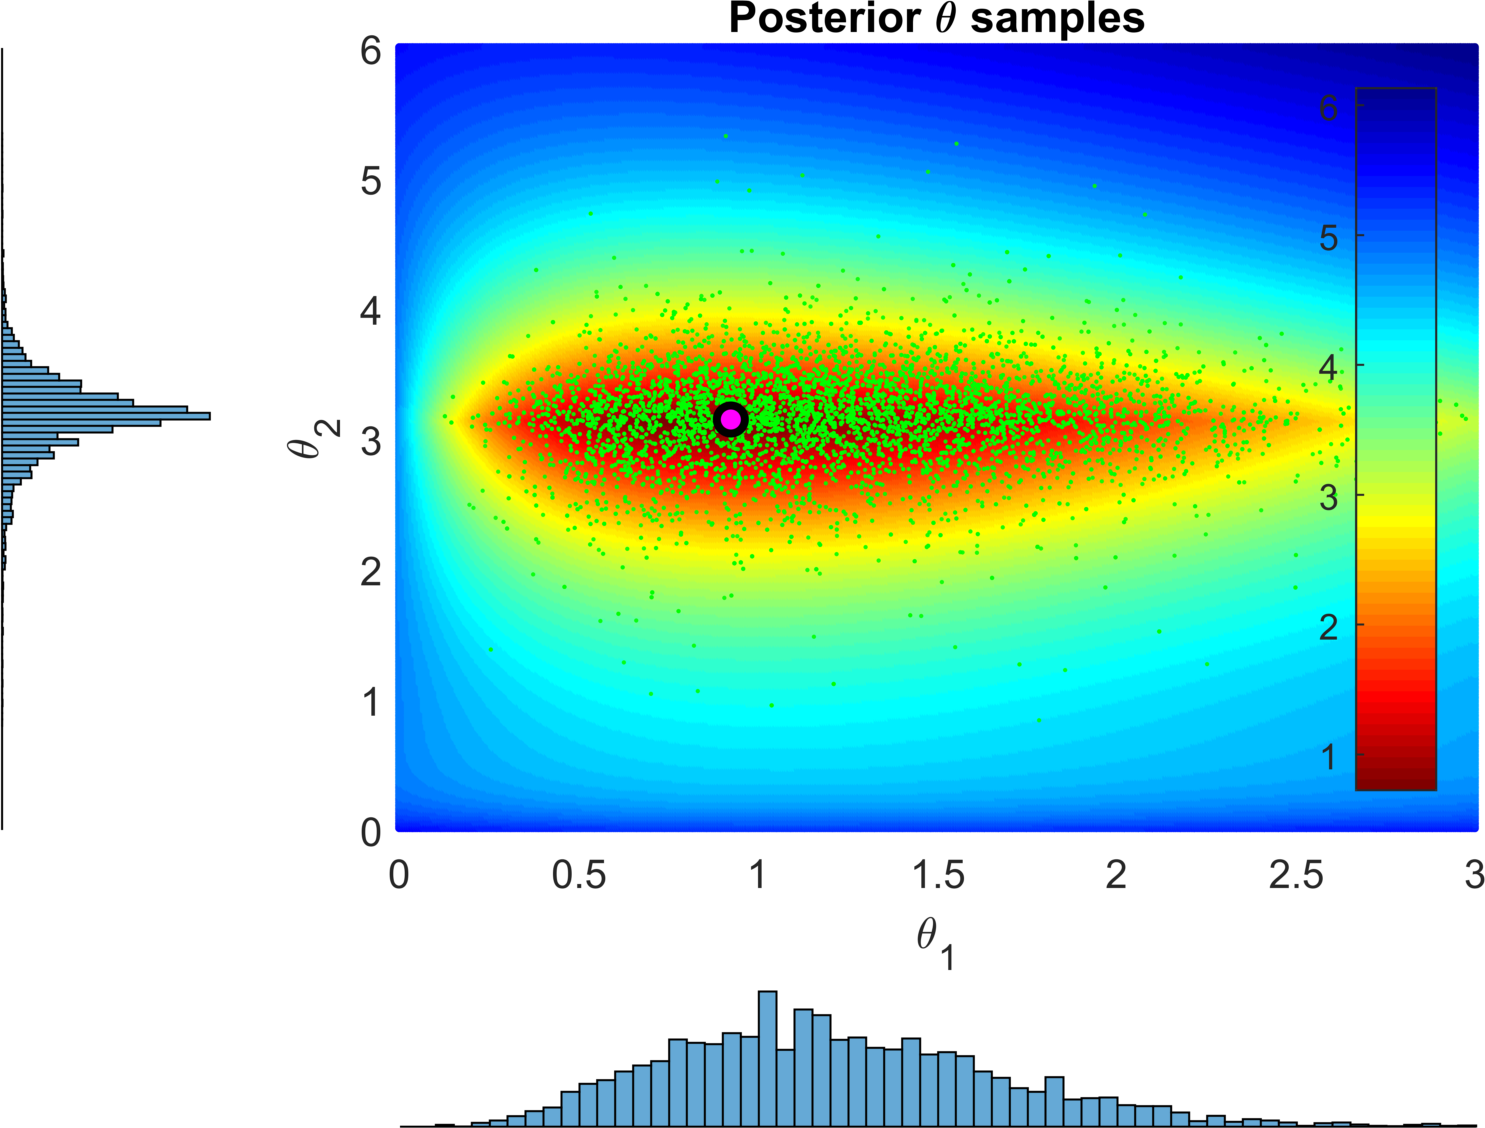
\includegraphics[width=0.95\linewidth]{FIG_post_theta_heatmap_desobs0_lambdadelta1}
%\caption{Example of a univariate Gaussian process}
\label{gp_ex}
\end{figure}

\begin{itemize}
\item 
The heatmap gives the Euclidean distance (on the standardized scale), at each point of the support of $\boldsymbol \theta$, of the model output at that point from the desired output $[0.71, 0.71, 17.92]$. 

\item The true optimum is shown as a purple dot. The green points are samples drawn via MCMC from the posterior distribution of $\boldsymbol\theta$, with marginal histograms also shown.
\end{itemize}



\end{alertblock}


%----------------------------------------------------------------------------------------

\end{column} % End of column 2.1

\begin{column}{\onecolwid}\vspace{-.6in} % The second column within column 2 (column 2.2)

%----------------------------------------------------------------------------------------
%	METHODS
%----------------------------------------------------------------------------------------

\begin{alertblock}{Wind turbine blade application}
We calibrate to find parameters for optimal performance and cost of a wind turbine blade of fixed geometry. We rely on a finite element simulator of the blade cost and performance.

\begin{figure}[h!]
\fbox{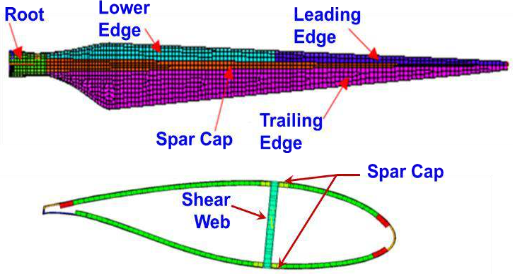
\includegraphics[width=0.65\linewidth]{blade3}}
%\caption{Wind turbine blade}
\label{blade}
\end{figure}

\vspace{-10mm}
\begin{itemize}
\item Calibration inputs: volume fraction, thickness of blade material (in mm). Control input: temperature (in Kelvin). Support of the calibration inputs is known to be $[0.2,0.6]\times[10,25]$.

%\item Control input is temperature.

\item Outputs are tip deflection, rotation, and cost; the design goal is to minimize these.

\item Model utilizes \texttt{ANSYS} simulation software; computation cost is too high for use in MCMC.

%\item \texttt{ANSYS} model cost too high for use in MCMC.

\end{itemize}
\end{alertblock}

\begin{alertblock}{Wind turbine blade results}

\begin{itemize}
\item The below figure gives the posterior distribution of the calibration inputs. The (uniform) prior distributions are given by the red dashed line.
\end{itemize}

\vspace{-5mm}
\begin{figure}[h!]
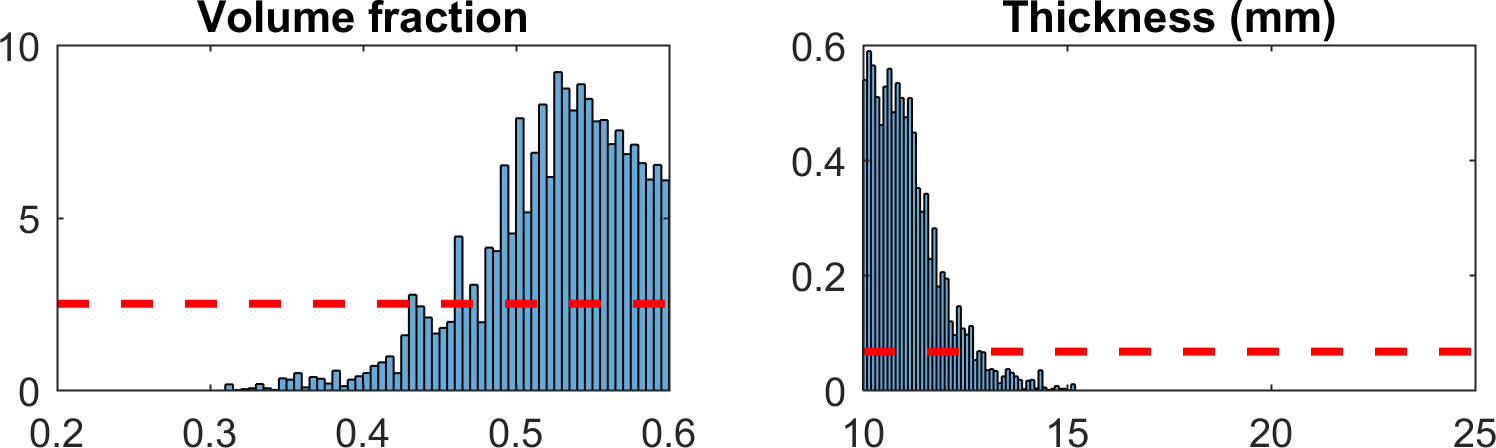
\includegraphics[width=.975\linewidth]{FIG_posterior_marginals_with_priors}
%\caption{Wind turbine blade}
\label{blade}
\end{figure}

\vspace{-8mm}
\begin{itemize}
\item The below figure gives the prior and posterior predictive distributions for the model. The dashed black lines show the desired observation.
\item Note that it is to be expected that, as seen here, the posterior predictive distribution does not peak at the desired observation, since the desired observation was intentionally selected to lie outside of the model range.
\end{itemize}

\begin{figure}[h!]
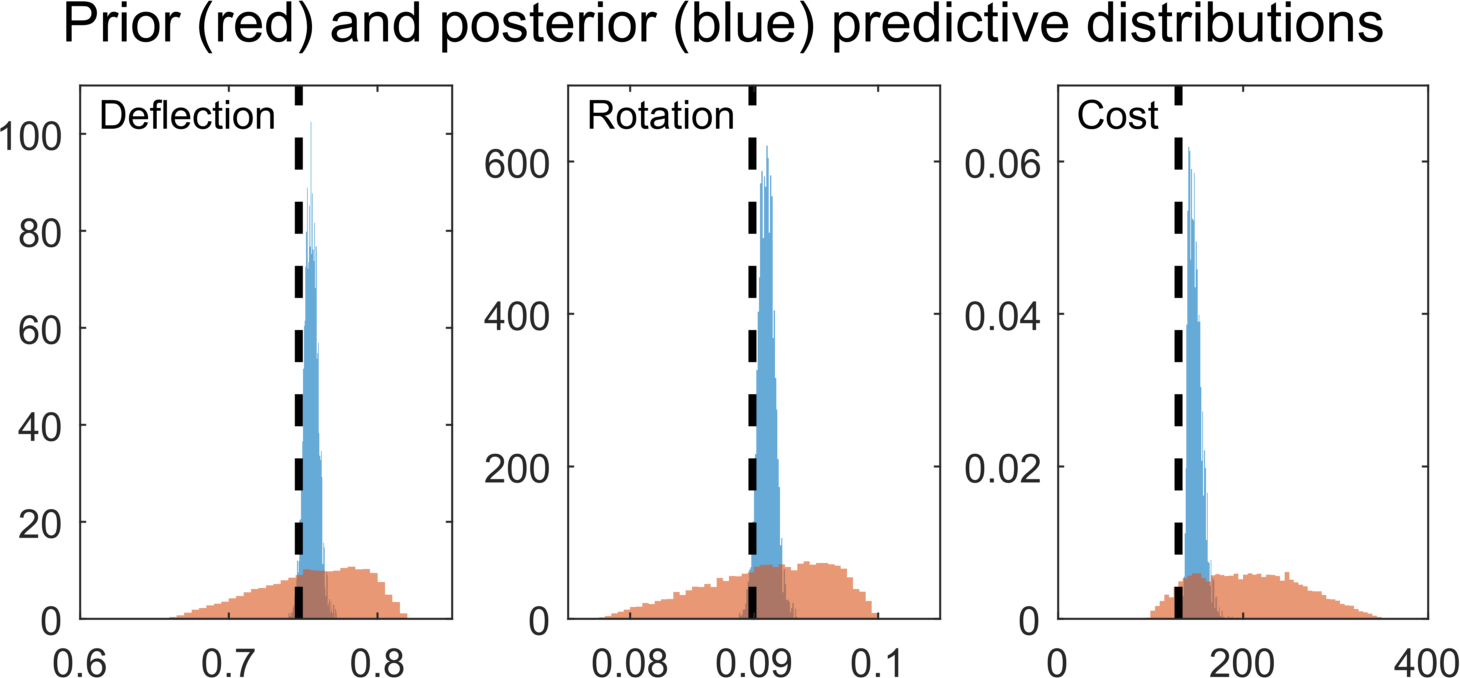
\includegraphics[width=.95\linewidth]{FIG_prior_vs_posterior_dist}
%\caption{Wind turbine blade}
\label{blade}
\end{figure}

%\vspace{-20mm}
%\end{itemize}

\end{alertblock}

%----------------------------------------------------------------------------------------

\end{column} % End of column 2.2

\end{columns} % End of the split of column 2 - any content after this will now take up 2 columns width

%----------------------------------------------------------------------------------------
%	IMPORTANT RESULT
%----------------------------------------------------------------------------------------

\setbeamercolor{block alerted title}{fg=Gray!15,bg=MidnightBlue!95} % Change the alert block title colors
\setbeamercolor{block alerted body}{fg=black,bg=MidnightBlue!10} % Change the alert block body colors



\setbeamercolor{block alerted title}{fg=Gray!15,bg=BrickRed!95} % Change the alert block title colors
\setbeamercolor{block alerted body}{fg=black,bg=BrickRed!05} % Change the alert block body colors


%----------------------------------------------------------------------------------------

\begin{columns}[t,totalwidth=\twocolwid] % Split up the two columns wide column again

\begin{column}{\onecolwid} % The second column within column 2 (column 2.2)

%----------------------------------------------------------------------------------------
%	RESULTS
%----------------------------------------------------------------------------------------
%
%\begin{alertblock}{Results}
%
%\begin{figure}
%
\includegraphics[width=0.8\linewidth]{placeholder.jpg}
%\caption{Figure caption}
%\end{figure}
%
%Nunc tempus venenatis facilisis. Curabitur suscipit consequat eros non porttitor. Sed a massa dolor, id ornare enim:
%
%\begin{table}
%\vspace{2ex}
%\begin{tabular}{l l l}
%\toprule
%\textbf{Treatments} & \textbf{Response 1} & \textbf{Response 2}\\
%\midrule
%Treatment 1 & 0.0003262 & 0.562 \\
%Treatment 2 & 0.0015681 & 0.910 \\
%Treatment 3 & 0.0009271 & 0.296 \\
%\bottomrule
%\end{tabular}
%\caption{Table caption}
%\end{table}
%
%\end{alertblock}

%----------------------------------------------------------------------------------------

\end{column} % End of column 2.2

\end{columns} % End of the split of column 2

\end{column} % End of the second column

\begin{column}{\sepwid}\end{column} % Empty spacer column

\begin{column}{\onecolwid} % The third column

%----------------------------------------------------------------------------------------
%	CONCLUSION
%----------------------------------------------------------------------------------------

\begin{alertblock}{Pareto bands}

\begin{itemize}

\item Rather than calibrating to a single set of desired observations, calibration can be performed at each point of a grid over $k-1$ of the $k$ model outputs.

\item This permits one to use the calibration procedure to get a comprehensive picture of the Pareto front of the model, complete with uncertainty bands.

\item This approach is illustrated here in the wind turbine application. For simplicity, only deflection and cost are considered. We drew a one-dimensional grid over the range of cost outputs from the model, and performed calibration at each point in the grid. 

\item At each point, we treat cost as known up to measurement error, and attempt to minimize deflection.

\item The below right plot shows the resulting estimate of the Pareto front for the model, with uncertainty bands.
\end{itemize}

\begin{figure}[h!]
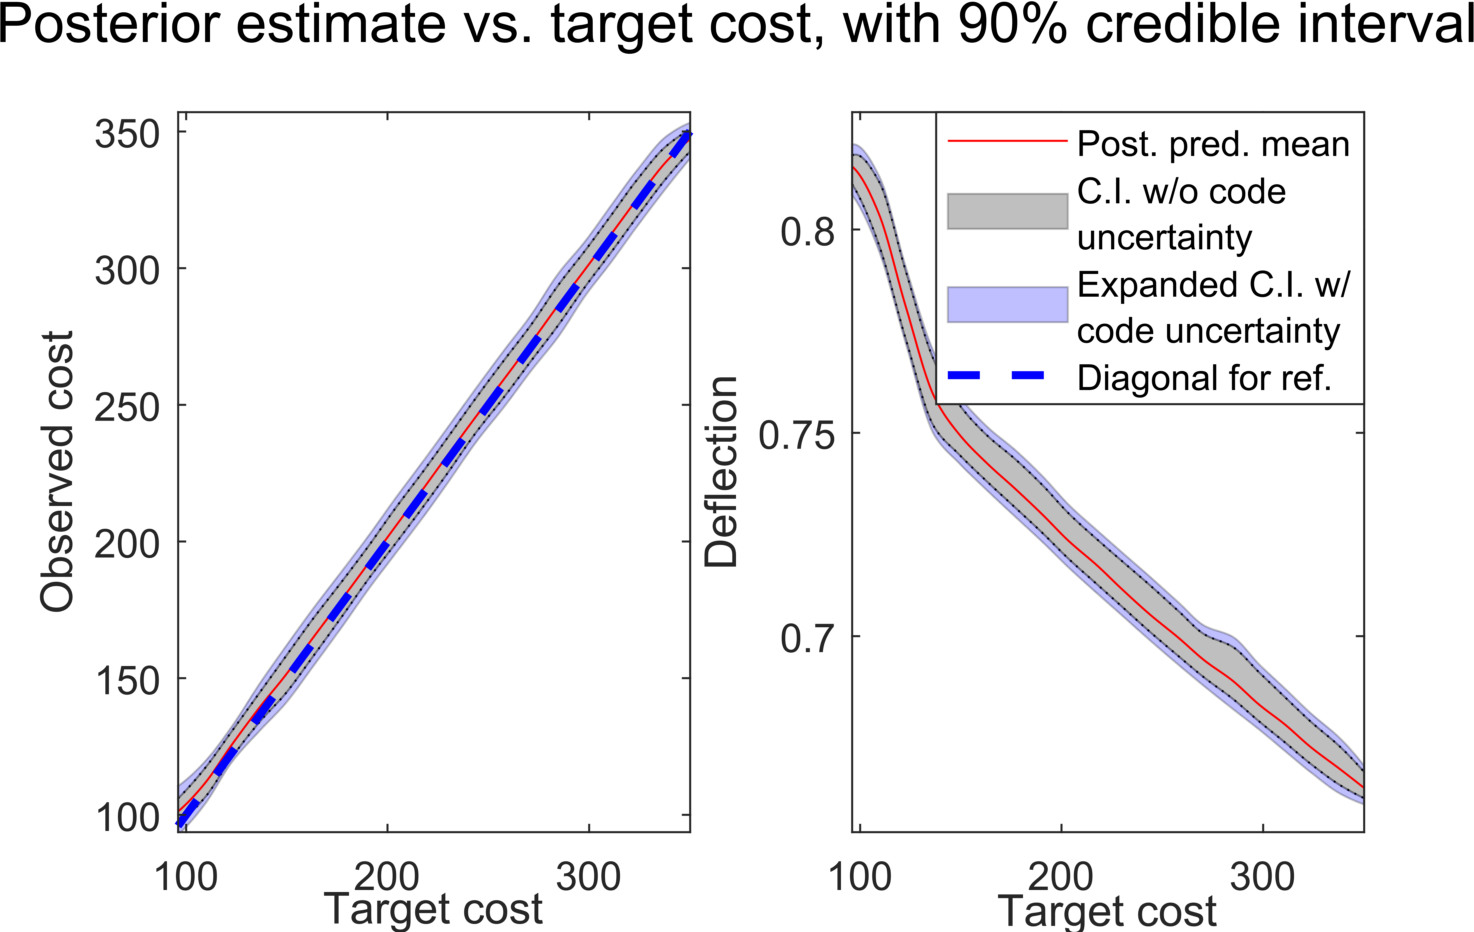
\includegraphics[width=\linewidth]{FIG_cost_grid_pareto_bands}
%\caption{Wind turbine blade}
\label{blade}
\end{figure}

\vspace{-18mm}
\begin{itemize}
\item The left plot is included to verify that the ``known'' cost was achieved in each calibration; i.e., that the target cost in the right plot faithfully represents the true cost.


\end{itemize}



\end{alertblock}

%----------------------------------------------------------------------------------------
%	ADDITIONAL INFORMATION
%----------------------------------------------------------------------------------------


%----------------------------------------------------------------------------------------
%	REFERENCES
%----------------------------------------------------------------------------------------

%\begin{alertblock}{References}
%
%\nocite{*} % Insert publications even if they are not cited in the poster
%\small{\bibliographystyle{unsrt}
%\bibliography{sample}\vspace{0.75in}}
%
%\end{alertblock}


%----------------------------------------------------------------------------------------
%	FUTURE COLLABORATION
%----------------------------------------------------------------------------------------

\setbeamercolor{alertblock alerted title}{fg=black,bg=norange} % Change the alert block title colors
\setbeamercolor{alertblock alerted body}{fg=black,bg=white} % Change the alert block body colors

\begin{alertblock}{Potential for future collaboration}

%\begin{itemize}
%\item Web: \href{http://www.university.edu/smithlab}{http://www.university.edu/smithlab}
%\item Email: \href{mailto:cehrett@clemson.edu}{cehrett@clemson.edu}
%\vspace{-15mm}
%\centering Carl Ehrett\\
%\centering Email: \href{mailto:cehrett@clemson.edu}{cehrett@clemson.edu}
%\item Phone: +1 (774) 234 7388
%\end{itemize}

\begin{itemize}
\item We are in search of new applications for the proposed methodology, particularly applications in which a posterior distribution is preferable to a point estimate of the optimum.

\item We intend to study the use of different sorts of code emulators (other than the GPs used here) for the proposed methodology.

\item We intend to compare the proposed methodology to more traditional means of optimization, with emphasis on uncertainty quantification.
\end{itemize}

%\vspace{-10mm}
\end{alertblock}

%----------------------------------------------------------------------------------------
%	ACKNOWLEDGEMENTS
%----------------------------------------------------------------------------------------

%\setbeamercolor{alertblock title}{fg=red,bg=white} % Change the block title color
%
%\begin{alertblock}{Acknowledgements}
%
%\small{\rmfamily{Nam mollis tristique neque eu luctus. Suspendisse rutrum congue nisi sed convallis. Aenean id neque dolor. Pellentesque habitant morbi tristique senectus et netus et malesuada fames ac turpis egestas.}} \\
%
%\end{alertblock}

\begin{alertblock}{References}
{
%\small
%\footnotesize
%\scriptsize
\tiny

\bibliographystyle{ieeetr}

\bibliography{poster}
}

\end{alertblock}



%----------------------------------------------------------------------------------------

\end{column} % End of the third column

\end{columns} % End of all the columns in the poster

\end{frame} % End of the enclosing frame

\end{document}
